\section{Sequential Circuits}
\label{sec:seq-cir}

Figure 5.1 shows a block diagram of a sequential circuit. It consists of a combinational circuit to which memory elements are connected to form a feedback path. The storage elements are devices capable of storing binary information. The binary information stored in these elements at any given time defines the state of the sequential circuit at that time.

\begin{figure}[H]
  \centering
  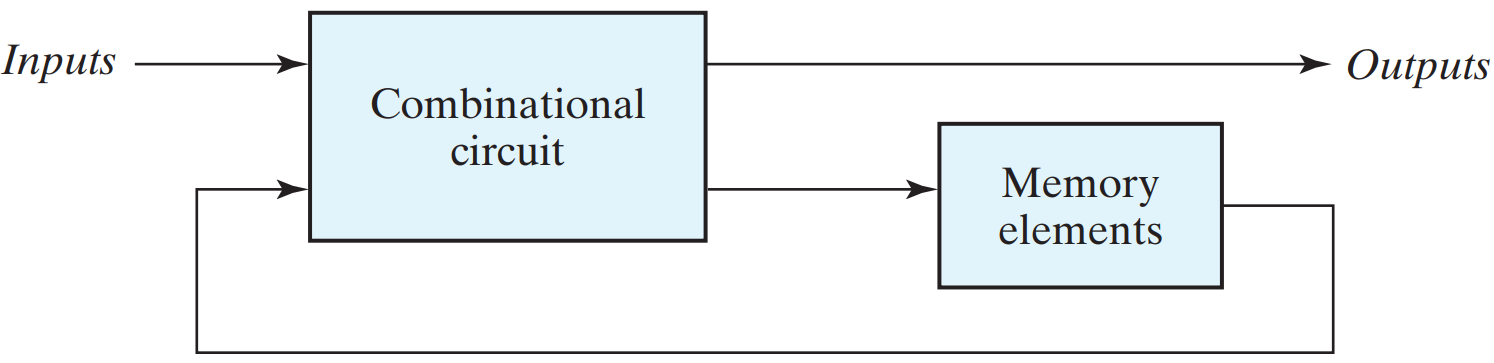
\includegraphics[width=\linewidth]{img/fig-5.1.png}
  \caption{Block diagram of sequential circuit}
  \label{fig:5.1}
\end{figure}

The block diagram demonstrates that the outputs in a sequential circuit are a function not only of the inputs but also of the present state of the storage elements. The next state of the storage elements is also a function of external inputs and the present state. Thus, \textit{\textbf{a sequential circuit is specified by a time sequence of inputs, outputs, and internal states}}.

There are two main types of sequential circuits, and their classification is a function of the timing of their signals:
\begin{itemize}
  \item A \textit{\textbf{synchronous} sequential circuit} is a system whose behavior can be defined from the knowledge of its signals at discrete instants of time.
  \item The behavior of an \textit{\textbf{asynchronous} sequential circuit} depends upon the input signals at any instant of  time \textit{and} the order in which the inputs change
\end{itemize}

A synchronous sequential circuit employs signals that affect the storage elements at only \textit{discrete instants of time}. Synchronization is achieved by a timing device called a \textit{clock generator}, which provides a clock signal having the form of a periodic sequence of clock pulses. In practice, the clock pulses determine when computational activity will occur within the circuit, and other signals (external inputs and otherwise) determine what changes will take place affecting the storage elements and the outputs.

Synchronous sequential circuits that use clock pulses to control storage elements are called \textit{clocked sequential circuits} and are the most 
frequently encountered type in practice. They are called \textit{synchronous circuits} because the activity within the circuit and the resulting updating of stored values is synchronized to the occurrence of clock pulses.

The storage elements (memory) used in clocked sequential circuits are called \textit{flip-flops}. A flip-flop is a binary storage device capable of storing one bit of information. In a stable state, the output of a flip-flop is either 0 or 1.

The block diagram of a synchronous clocked sequential circuit is shown in  Fig. 2. 
\begin{figure}[H]
  \centering
  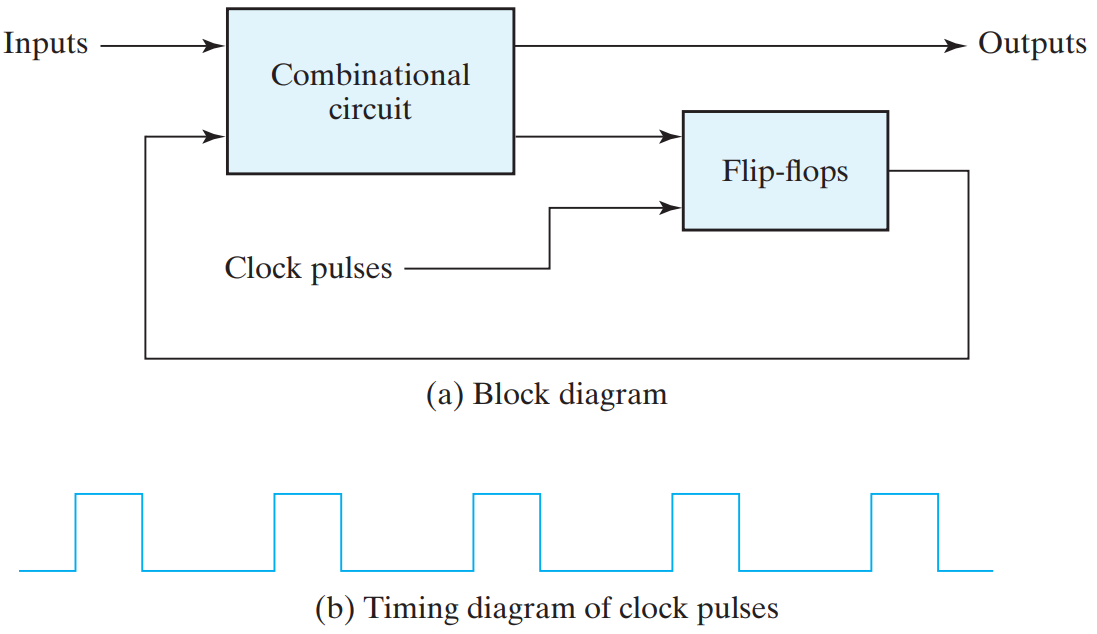
\includegraphics[width=\linewidth]{img/fig-5.2.png}
  \caption{Synchronous clocked sequential circuit}
  \label{fig:5.2}
\end{figure}

\begin{itemize}
  \item The \textit{outputs} are formed by a \textit{combinational logic function of the inputs to the circuit or the values stored in the flip-flops (or both)}. 
  \item The \textit{value that is stored in a flip-flop} when the clock pulse occurs is also determined by \textit{the inputs to the circuit or the values presently stored in the flip-flop (or both)}.
  \item The \textit{new value is stored} (i.e., the flip-flop is \textit{updated}) when a pulse of the clock signal occurs. Prior to the occurrence of the clock pulse, the combinational logic forming the next value of the flip-flop must have reached a stable value.
\end{itemize}

\begin{practice}{Practice Exercise 5.1}
Describe the fundamental difference between the output of a combinational circuit and the output of a sequential circuit. \\

\textbf{Answer:} 
The output of a combinational circuit depends on only the inputs to the circuit; the output of a sequential circuit depends on the inputs to the circuit and the present state of the storage elements.
\end{practice}
